\documentclass{mise_en_page}

\usepackage{booktabs} % Required for the \toprule, \midrule and \bottomrule lines
\usepackage{array}
\usepackage{float}

\projet{Projet Ingéniérie}
\equipe{H4314}
\responsable{Tristan Delizy}
\redacteurs{Arnaud Lahache} % Optionnel
\titre{Plan d'Assurance Qualité Projet}
\version{1.3}
\objet{Ce dossier a pour but de décrire les dispositions prises en matière d’assurance de la qualité pour le projet COPEVUE-MONIT}
\etat{ébauche} %draft, non relu, non validé, validé

\begin{document}

\maketitle

\begin{historique}
    \histo{1.0}{23/01/2012}{Initialisation du document}
    \histo{1.1}{30/01/2012}{Début de la mise en page}
    \histo{1.2}{06/02/2012}{Finalisation de l'ébauche}
    \histo{1.3}{09/02/2012}{Validation de l'ébauche}
\end{historique}

\newpage

\tableofcontents

\section{Objet et caractéristiques du PAQP}

\subsection{Objectifs}
L’objectif du PAQP est de décrire les dispositions prises en matière d’assurance de la qualité pour le projet COPEVUE-MONIT. Ces dispositions seront à respecter pour l'ensemble des sous-projets. Cependant dans le cas où certains sous-projets auraient des contraintes spécifiques, ils pourront disposer de leurs propres démarches qualités spécifique dictées dans des PAQL au niveau \emph{Logiciel}.

Ce dossier aura donc pour but de décrire les grandes lignes d'assurance qulité afin d'assurer à la MOA une certaine qualité des livrables pour l'ensemble du projet.

\subsection{Documents applicables et de référence}

\subsubsection{Documents de référence}

\begin{description}
	\item[GLOSSAIRE / GL / glossaire] Glossaire commun à l'ensemble du projet MIME.
	\item[3IF / Génie Logiciel] Cours 3IF sur le Génie Logiciel par Régis Aubry
	\item[4IF / Qualité] Cours 4IF sur la qualité par Régis Aubry
\end{description}

\subsubsection{Documents applicables}

\begin{description}
	\item[QL / GDOC / gestionDocumentation] Gestion de la documentation générale de notre société. Ce dossier déjà réalisé servira de base à la gestion de documentation du PAQP.
\end{description}

\subsection{Terminologie et glossaire}

Les terminologies utilisées dans ce dossier sont spécifiques au projet COPEVUE-MONIT. Afin de pouvoir séparer les terminologies liées au projet général, ainsi que les terminologies seulement en relation avec la démarche qualité du projet, nous avons constitué deux documents constituant les glossaires vers lesquels vous pourrez vous référer :

\begin{description}
	\item[GLOSSAIRE / QL / glossaireQualite ] Glossaire spécifique à la démarche qualité du projet.
	\item[GLOSSAIRE / GL / glossaire ] Glossaire commun à l'ensemble du projet COPEVUE-MONIT.
\end{description}

Vous pouvez donc vous référer à l'ensemble de ces documents pour tous les points concernants les terminaisons ainsi que le glossaire.

\section{Objectifs et engagements qualité du projet}

\subsection{Exigences non fonctionelles}

L'appel d'offre émis par la COPEVUE nous a permis de dégager un ensemble d'exigences non fonctionnelles qui formeront les principaux objectifs en dispositions de qualité du projet COPEVUE-MONIT.

\begin{description}
	\item[INTÉGRATION DE L'EXISTANT] réutiliser les composants des systèmes présents sur les différents sites
	\item[ROBUSTESSE] Éviter les coupures suite à des causes environnementales, résistance aux conditions extrêmes
	\item[FIABILITÉ] Autonomie suffisante, pas de bloquage du système global
	\item[ÉVOLUTIVITÉ ET MAINTENABILITÉ] Intéropérabilité avec les autres applications, améliorations du système facilitées, scalabilité.
	\item[LIMITATION TECHNOLOGIQUES] Matériel GPS et GPRS dont le fonctionnement n'est pas à 100\% Maîtrisé.
	\item[GÉNÉRICITÉ] Utilisation de progiciels, réutilisation des composants pour d'autres systèmes, paramétrage.
	\item[ERGONOMIE] Utilisation du système par des non informaticiens, interface homme-machine différentes selon l'utilisateur.
	\item[TRACABILITÉ] Log et traces des activités du système stockées sur un période de 2 ans minimum.
\end{description}

\subsection{Déclinaison en engagements qualité}

\begin{description}
	\item[Fiabilité]
		Ensemble d'attributs portant sur l'aptitude du logiciel à maintenir soon niveau de service dans des conditions précises et pendant une période déterminée
		\begin{itemize}
			\item Maturité
			\item Tolérance aux fautes
			\item Possibilité de récupération
		\end{itemize}
	\item[Facilité d'utilisation]
		Ensemble d'attributs portant sur l'effort nécéssaire pour l'utilisation et sur l'évaluation individulle de cette utilisation par un ensemble défini ou implicite d'utilisateurs
		\begin{itemize}
			\item Facilité de compréhension
			\item Facilité d'apprentissage
			\item Facilité d'exploitation
		\end{itemize}
	\item[Rendement]
		Ensemble d'attributs portant sur le rapport entre le niveau de service d'un logiciel et la quantité de ressource utilisées, dans des conditions déterminées
		\begin{itemize}
			\item Comportement vis-à-vis du temps
			\item Comportement vis-à-vis des ressources
			\item Autonomie
		\end{itemize}
	\item[Maintenabilité]
		Ensemble d'attributs portant sur l'effort nécessaire pour faire des modifications données
		\begin{itemize}
			\item Facilité d'analyse
			\item Facilité de modification
			\item Stabilité
			\item Facilité de test
		\end{itemize}
\end{description}

\section{Conduite de projet}

\subsection{Présentation des relations et des rôles}

\subsubsection{Équipe SIMME}

Les responsabilités ont été distribuées au début du projet. Un chef de projet a été nommé ainsi qu'un responsable qualité. Le reste de l'équipe compose le GEI (Groupe d'Etude Informatique) (voir le tableau \ref{tab_equipe} plus bas.)

La responsabilité du chef de projet est de mener le projet à bien et de gérer son équipe, mais également de garder un \oe{}il sur la cohérence du contenu des différents dossiers. Le responsable qualité aura pour tâche d'assurer une certaine cohérence formelle des livrables rendus mais également de mettre en place une démarche qualité au niveau projet et sous-projet.

La responsabilité du GEI s'étend de l'étude jusqu'à la rédaction complète des drafts et des livrables des différents dossiers nécessaires au projet. C'est le GEI qui délivrera grâce à ses recherches la solution proposée.

\begin{table}[h]
	\centering
	\begin{tabular}{l r}
		\toprule
		\textbf{Prénom et Nom} & \textbf{Rôle dans l'équipe}\\
		\toprule
		Tristan Delezy & Chef de Projet \\
		Arnaud Lahache & Responsable qualité \\
		\midrule
		Jérémy Tuloup & GEI \\
		Pierre Lulé & GEI \\
		Léo Lefebvre & GEI \\
		Sébastien Laurent & GEI \\
		\bottomrule
	\end{tabular}
	\caption{\label{tab_equipe} Présentation de l'équipe}
\end{table}

\subsubsection{Organisation du projet SIMME}

\begin{figure}[H]
	\centering
	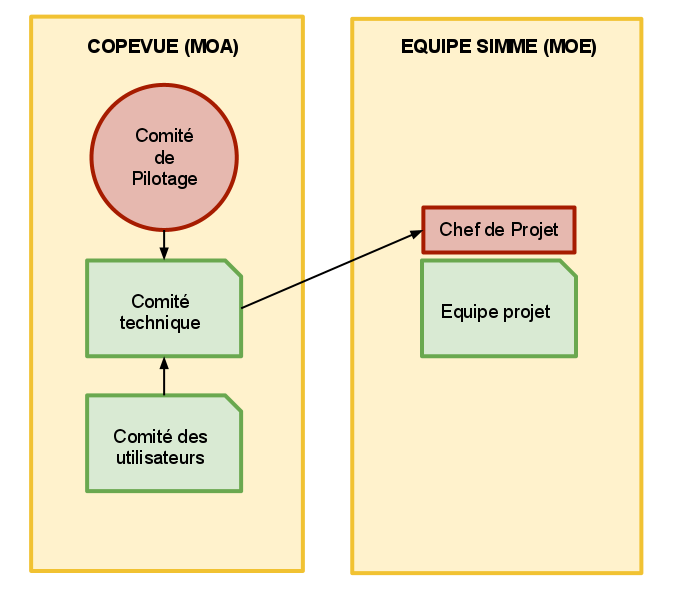
\includegraphics[width=150mm]{MOASIMME.png}
	\caption{\label{MOA} Constitution de la MOA (COPEVUE) et de la MOE (Équipe SIMME)}
\end{figure}

\begin{description}
	\item[MOA]
		La Maîtrise d'Ouvrage (MOA) représente la COPEVUE : elle est composée d'un comité de pilotage, d'un comité technique et d'un comité des utilisateurs. (Cf. Fig. \ref{MOA})
	\item[MOE]
		La Maîtrise d'Ouvrage (MOE) désigne l'équipe SIMME décrite çi-dessus. Le Chef de Projet (Tristan Delezy) a un rôle de représentation face à la MOA.
\end{description}

\begin{figure}[H]
	\centering
	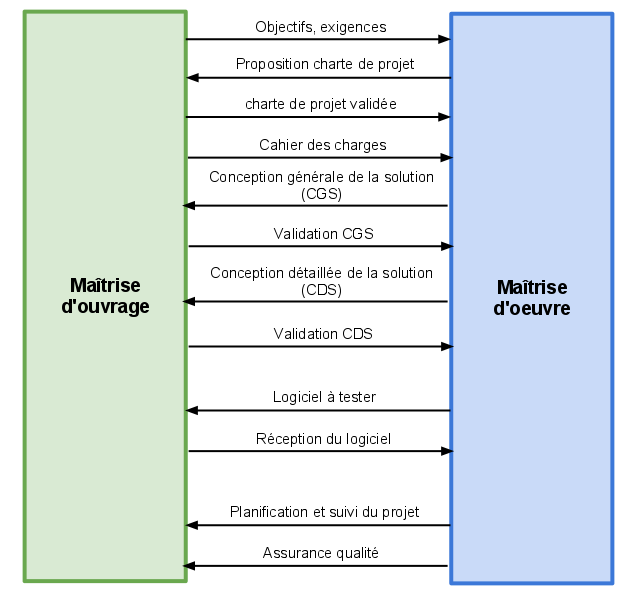
\includegraphics[width=150mm]{MOAMOE.png}
	\caption{\label{MOE} Relations entre MOA et MOE}
\end{figure}

\subsubsection{Organisation des sous-projets}

L'ampleur du projet COPEVUE-MONIT (également appelé SIMME dans notre fiche commerciale) nous amène à découper ce dernier en plusieurs sous-projets. Le développement de ces sous-projets (expliqué plus bas) entraîne de nouvelles relations MOA-MOE, avec cette-fois-çi l'équipe SIMME dans le rôle de la MOA.

Suivant les sous-projets développés lors du projet COPEVUE-MONIT, le développement pourra se faire en interne ou en externe. Dans tous les cas, l'équipe MOE constituée pour réaliser le sous-projet devra travailler en collaboration étroite avec la MOA (Équipe SIMME). Les relations entre MOA et MOE seront identiques des relations entre L'équipe SIMME et la COPEVUE (Cf. Fig. \ref{MOE}), et auront pour but de mener à bien la réalisation des sous-projets.

La MOA aura pour charge de rédiger les cahier des charges et PAQL de chaque sous-projets. Les retours de la MOE sont très importants pour savoir si ces derniers ont bien pris en compte tous les besoins fonctionnels et no fonctionnelles. Des revues seront également régulièrement organisées afin de pouvoir vérifier l'avancement des sous-projets. Les revues seront organisées selon le planning durant toute la durée de l'exécution du projet.

Le commanditaire de la MOA sera Tristan Delezy, chef de projet de l'équipe SIMME. Un représentant de la MOE de chaque sous-projet sera nommé afin de mettre en place un interlocuteur unique lors des relations entre MOA et MOE.

\subsection{Démarche de développement SYSTÈME}

L'ampleur du projet COPEVUE-MONIT et son organisation en sous-projets nous amène à considérer sa démarche de développement au niveau \emph{SYSTÈME}.

Les sous-projets induits auront leur propre démarche de développment énoncée dans leur PAQL. Les phases de spécification, conception et d'intégration au niveau Projet doivent cependant respecter une démarche de type \emph{Cycle en V}.

\begin{figure}[H]
	\centering
	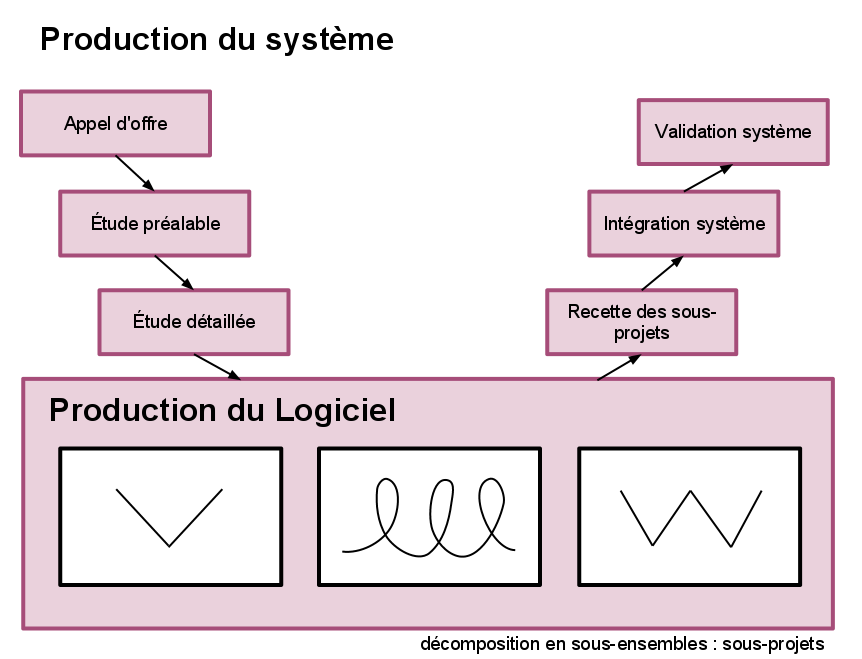
\includegraphics[width=150mm]{DEMARCHE.png}
	\caption{\label{DEMARCHE} Démarche de développement au niveau SYSTÈME}
\end{figure}

\section{Gestion de la documentation}

La gestion de la documentation du projet COPEVUE-MONIT applique les principes énoncés dans le document \emph{QL / GDOC / gestionDocumentation} présent dans les documents applicables. Vous pouvez donc vous y référer.

\begin{description}
	\item[QL / GDOC / gestionDocumentation] Gestion de la documentation générale de notre société. Ce dossier déjà réalisé servira de base à la gestion de documentation du PAQP.
\end{description}

\section{Gestion de la configuration}

\subsection{Objectifs}

La gestion de la configuration a pour but de poser des normes et des procédures qui permettent aux équipes du projet d'obtenir une certaine cohérence dans le temps sur les documents et les composants. Elle permet d'accéder à tous les composants du projet à n'importe quel moment du développement.

Les codes sources, la documentation ainsi que les bases de données ou fichier utilisées par l'application font tous l'objet de la gestion de configuration.

\subsection{Gestion des versions et des révisions}

Afin d'identifier un composant dans le temps, un identifiant de version sera assigné à cet élément de la forme : \emph{\#Numéro de version\#.\#Numéro de révision\#}

\begin{description}
	\item[Numéro de version]
		correspond à la version du logiciel ou de l'élément, incrémenté à chaque jalon franchi par le composant.
	\item[Numéro de révision]
		identifie la révision effectuée pour cette version du composant. La révision est incrémentée à chaque modification de l'élement. Elle est réinitialisée à 0 lorsqu'on change de version.
\end{description}

\subsection{Arbre de configuration du système}

\begin{figure}[H]
	\centering
	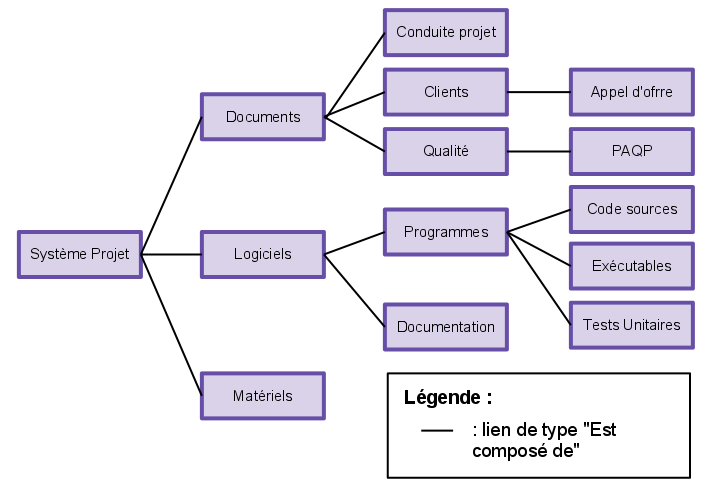
\includegraphics[width=150mm]{CONF.png}
	\caption{\label{CONF} Arbre de configuration du système dans le cadre du projet COPEVUE-MONIT}
\end{figure}

\section{Gestion des modifications}

\subsection{Identification des modifications}

La gestion des modifications se décompose en deux parties distinctes :

\begin{description}
	\item[Gestion des évolutions]
		Les évolutions sont des changements fonctionnels non définis dans une expression des besoins ou un cahier des charges suite à une \emph{Demande d'Évolution} (DE).
	\item[Gestion des corrections]
		Les corrections sont des adaptations prises en comptes suite à un \emph{Rapport d'Anomalie} (RA), signalant une défaillance ou d'une non conformité.
\end{description}

\subsection{Procédure de gestion des évolutions}

\begin{figure}[H]
	\centering
	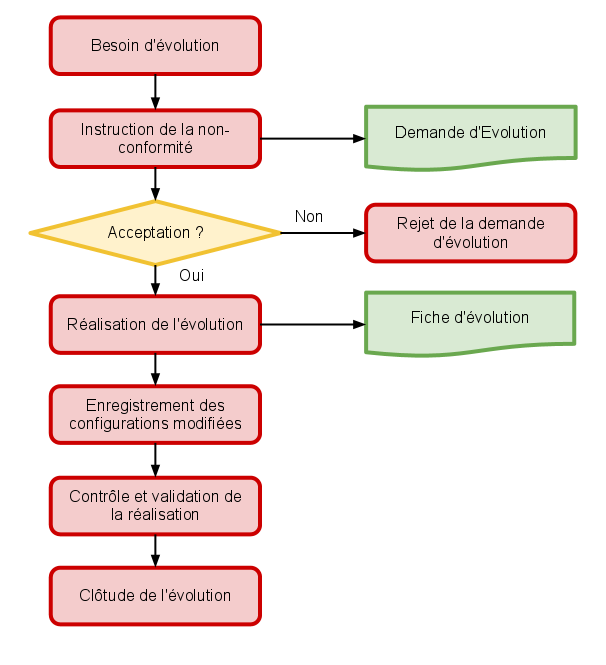
\includegraphics[width=150mm]{evol.png}
	\caption{\label{evol} Procédure de gestion des évolutions}
\end{figure}

\subsection{Procédure de gestion des corrections}

\begin{figure}[H]
	\centering
	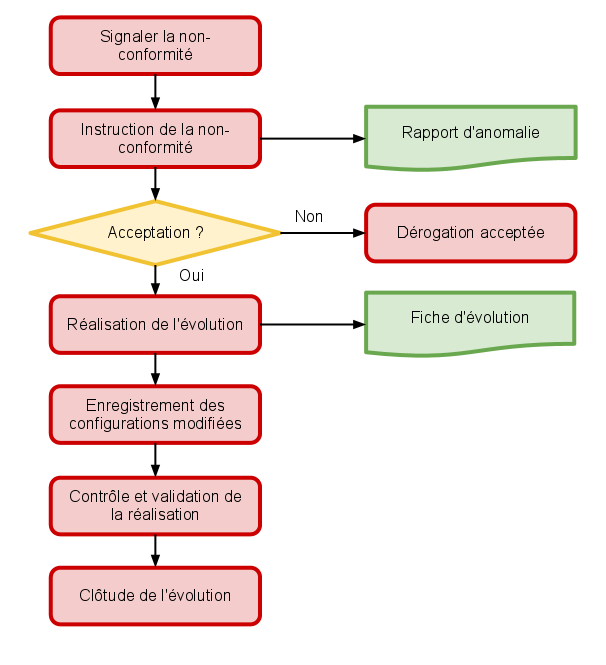
\includegraphics[width=150mm]{correction.png}
	\caption{\label{evol} Procédure de gestion des corrections}
\end{figure}

\end{document}
